\documentclass[12pt]{amsart}

\topmargin=-0.4in \oddsidemargin=0.2in \evensidemargin=0.2in
\textwidth=6.2in \textheight=9in

\usepackage{amssymb,amsfonts,amsmath,amsthm,epsfig,tikz,bm,color}
%\usepackage{showkeys}
%=================================================
\def\dfrac{\displaystyle\frac} \def\ovl{\overline} \def\Int{\displaystyle\int}
\def\Rm#1{\lowercase\expandafter{\romannumeral#1}}
\def\for{\forall~} \def\exi{\exists~} \def\c{\subseteq}
\def\iif{\Leftrightarrow} \def\Rto{\Rightarrow} \def\Lto{\Leftarrow}
\def\oo{\infty} \def\pa{\partial} \def\rto{\rightarrow} \def\mto{\mapsto}
\def\ug{\triangle} \def\dg{\nabla} \def\lg{\langle} \def\rg{\rangle}\def\Ga{\Gamma}\def\Core{{\sf Core}}
%=================================================
\def\T{\Gamma}  \def\D{\Delta} \def\Th{\Theta}
\def\Lmd{\Lambda} \def\E{\Sigma} \def\O{\Omega}
\def\a{\alpha} \def\b{\beta} \def\g{\gamma} \def\d{\delta} \def\e{\varepsilon}
\def\r{\rho} \def\o{\sigma} \def\t{\tau} \def\w{\omega} \def\k{\kappa}
\def\th{\theta} \def\lmd{\lambda} \def\ph{\varphi} \def\z{\zeta} \def\ti{\tilde} \def\SS{{\rm S}}\def\DD{{\rm D}}
%=================================================
\def\A{$A$} \def\G{$G$} \def\H{$H$} \def\K{$K$} \def\M{$M$} \def\N{$N$}
\def\P{$P$} \def\Q{$Q$} \def\R{$R$} \def\V{$V$} \def\X{$X$} \def\Y{$Y$}
\def\bfA{{\bf A}} \def\rmD{{\rm D}} \def\bfS{{\bf S}} \def\bfK{{\bf K}}
\def\bfM{{\bf M}} \def\bbZ{{\Bbb Z}} \def\GL{{\bf GL}} \def\C{Cayley\,}
\def\CS{Cay(G,S)} \def\CT{Cay(G,T)} \def\Iso{Iso(S,T)} \def\B{$B$}\def\ZZ{\mathbb Z}
%=================================================
\def\oa{\ovl A} \def\og{\ovl G} \def\oh{\ovl H} \def\ob{\ovl B} \def\oq{\ovl Q}
\def\oc{\ovl C} \def\ok{\ovl K} \def\ol{\ovl L} \def\om{\ovl M} \def\on{\ovl N}
\def\op{\ovl P} \def\oR{\ovl R} \def\os{\ovl S} \def\ot{\ovl T} \def\ou{\ovl U}
\def\ov{\ovl V} \def\ow{\ovl W} \def\ox{\ovl X} \def\oT{\ovl\T}
%=================================================
\def\di{\bigm|} \def\Di{\Bigm|} \def\nd{\mathrel{\bigm|\kern-.7em/}}
\def\Nd{\mathrel{\not\,\Bigm|}} \def\edi{\bigm|\bigm|}
\def\m{\medskip} \def\l{\noindent} \def\x{$\!\,$} \def\J{$-\!\,$}
%=================================================
\def\Hom{\hbox{\rm Hom}} \def\Aut{\hbox{\rm Aut}} \def\Inn{\hbox{\rm Inn}}  \def\OD{\hbox{\rm OD}}
\def\Syl{\hbox{\rm Syl}} \def\Sym{\hbox{\rm Sym}} \def\Alt{\hbox{\rm Alt}}
\def\Ker{\hbox{\rm Ker}} \def\fix{\hbox{\rm fix}} \def\mod{\hbox{\rm mod}\,}
\def\GL{\hbox{\rm GL}} \def\GF{\hbox{\rm GF}} \def\PG{\hbox{\rm PG}}
\def\pgl{\hbox{\bf PGL}} \def\psl{{\bf PSL}} \def\psu{{\bf PSU}}
\def\Cay{\hbox{\rm Cay}} \def\Mult{\hbox{\rm Mult}} \def\Iso{\hbox{\rm Iso}}
\def\Val{\hbox{\rm Val}} \def\Sab{\hbox{\rm Sab}} \def\supp{\hbox{\rm supp}}
\def\qed{\hfill $\Box$} \def\qqed{\qed\vspace{3truemm}}
\def\CS{\Cay(G,S)} \def\CT{\Cay(G,T)} \def\Arc{\hbox{\rm Arc}} \def\Cos{{\rm Cos}}
\def\fs{\footnotesize} \def\bbZ{{\Bbb Z}} \def\bbQ{{\Bbb Q}} \def\bbN{{\Bbb N}}
\def\Hol{\hbox{\rm Hol}} \def\rad{\hbox{\rm rad}}
%=================================================

\newtheorem{thm}{Theorem}[section]
\newtheorem{cor}[thm]{Corollary}
\newtheorem{lem}[thm]{Lemma}
\def\theequation{\thesection.\arabic{equation}}
\makeatletter \@addtoreset{equation}{section}
\newtheorem{rmk}{Remark}[section]
\newtheorem*{rmk1}{Remark}
\newtheorem{que}[thm]{Question}
\newtheorem{pro}[thm]{Proposition}
\newtheorem{con}[thm]{Condition}
\newtheorem{rem}[thm]{\it Remarks}
\newtheorem{defi}[thm]{Definition}
\newtheorem{exa}{\it Example}
\newtheorem{obs}{\it Observation}
\newtheorem{prob}[thm]{Problem}
\def\pf{\noindent {\it Proof.\ }}
\def\qed{\ifmmode\square\else\nolinebreak\hfill
$\Box$\fi\par\vskip12pt}






\begin{document}


\title[Orbits and Stabilizers]
{Orbits and Stabilizers}%
\maketitle

\l Exercises

\l 1. Let $G$ be a group acting transitively on a set $\O$, $H$ be a subgroup of $G$ and $G_{\a}$ be a point stabilizer of $G$. Show that $G=G_{\a}H\iif G=HG_{\a}\iif H$ is transitive. In particular, the only transitive subgroup of $G$ containing $G_{\a}$ is $G$ itself. (Frattini Arguement)
\m

\pf We just need to prove $G=G_{\a}H\iif H$ is transitive. \\
($\Rto$) Since $G$ acts transitively on $\O$, there exists $g\in G$ such that ${\a}^g=\b$ for any $\b\in \O$.
Recall that $G=G_{\a}H$, then $g=xh$ where $x\in G_{\a}$ and $h\in H$.
We have that ${\a}^(xh)={\a}^h=\b$, then $H$ is transitive.\\
($\Lto$) Obviously, $G_{\a}H\le G$ and $G_{\a}\cap H=H_{\a}$.
Since $G$ and $H$ is transitive on $\O$, we have $|G:G_{\a}|=|H:H_{\a}|=|\O|$.
Then
\begin{align*}
 |G_{\a}H|=\frac{|G_{\a}||H|}{|G_{\a}\cap H|}=\frac{|G_{\a}||H|}{|H_{\a}|}=|G_{\a}||\O|=|G|,
\end{align*}
that is, $G=G_{\a}H$.

If there is a transitive subgroup $K$ of $G$ which contains $G_{\a}$, then we have $G=G_{\a}K=K$ by the above proof.
Thus, the only transitive subgroup of $G$ containing $G_{\a}$ is $G$ itself.

\m
\m

\l 2. Show that the action of the group of symmetries of the cube on the set of six faces of the cube is transitive, and deduce that the group of symmetries has a subgroup of index 6.
\m

\pf Let $G$ be the group of symmetries of the cube and $\O$ be the set of six faces of the cube.
Choosing $\a=\{1,2,3,4\}$ is a face in Figure~\ref{figure1}.
Then there exist $g_1=(18)(27)$, $g_2=(15)(26)(48)(37)$, $g_3=(45)(36)$, $g_4=(25)(38)$, $g_5=(16)(47)$, such that $\a$ is moved to be the remaining five faces in $\O$, respectively.
Thus, $G$ is transitive on $\O$.

Since $G$ is transitive on $\O$, we have $|G:G_{\a}|=|\O|=6$. 
Thus, $G_{\a}$ is a subgroup of index 6.

\begin{figure}[htb]
\begin{center}
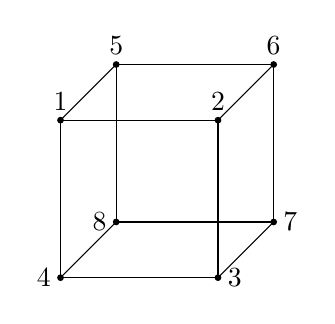
\begin{tikzpicture}(100,100)(20,20)
\thicklines
\draw(0,0)--(2,0);
\draw(0,0)--(0,2);
\draw(0,0)--(0.707,0.707);
\draw(2,0)--(2,2);
\draw(2,0)--(2.707,0.707);
\draw(0,2)--(2,2);
\draw(0,2)--(0.707,2.707);
\draw(2,2)--(2.707,2.707);
\draw(0.707,0.707)--(0.707,2.707);
\draw(0.707,0.707)--(2.707,0.707);
\draw(2.707,0.707)--(2.707,2.707);
\draw(0.707,2.707)--(2.707,2.707);

\draw(0,2)node [above]{1};
\draw(2,2)node [above]{2};
\draw(2,0)node [right]{3};
\draw(0,0)node [left]{4};
\draw(0.707,2.707)node [above]{5};
\draw(2.707,2.707)node [above]{6};
\draw(2.707,0.707)node [right]{7};
\draw(0.707,0.707)node [left]{8};

\filldraw [black] (0,2) circle (1pt);
\filldraw [black] (2,2) circle (1pt);
\filldraw [black] (2,0) circle (1pt);
\filldraw [black] (0,0) circle (1pt);
\filldraw [black] (0.707,2.707) circle (1pt);
\filldraw [black] (2.707,2.707) circle (1pt);
\filldraw [black] (2.707,0.707) circle (1pt);
\filldraw [black] (0.707,0.707) circle (1pt);

\end{tikzpicture}
\end{center}
\caption{The Cube}
\label{figure1}
\end{figure}

\m
\m

\l 3. Let $H=G_1$ be the group of symmetries of the cube which fix vertex 1. What are the orbits of $H$ on the set of 12 edges of the cube?
\m

\pf Let $\O$ be the set of 12 edges of the cube and $H$ is intransitive on $\O$. By Figure~\ref{figure1}, we have
$\{1,2\}^H=\{\{1,2\},\{1,5\},\{1,4\}\}$;
$\{2,3\}^H=\{\{2,3\},\{3,4\},\{5,6\},\{5,8\},\{4,8\},\{2,6\}\}$;
$\{7,8\}^H=\{\{7,8\},\{6,7\},\{3,7\}\}$.

\m
\m

\l 4. Calculate the order of the symmetry group of the regular dodecahedron.
\m

\pf Let $\O$ be the set of the edges of the regular dodecahedron and $\a\in \O$, then $|\O|=12$ and $|G_{\a}|=10$.
Since $G$ is transitive on $\O$, we have $|G|=|G_{\a}||{\a}^G|=|G_{\a}||\O|=12\cdot 10=120$.





\end{document}
